\section{Développement python}

Une fois la configuration de Jenkins terminée, nous pouvons entamer l’implémentation du code du projet PowerGrid. L'objectif principal de ce projet étant de nous familiariser avec les outils de gestion de projets, il est logique, dans ce contexte, de répartir les tâches de développement logiciel entre les membres de l’équipe.
Ainsi, chacun de nous peut se concentrer sur différentes fonctions à implémenter, en travaillant sur nos branches respectives \textit{dev-noe} et \textit{dev-leah}.
Cette approche permet de paralléliser le travail, et une fois nos tâches terminées, nous pourrons fusionner nos branches pour obtenir une version unique et consolidée, intégrant nos implémentations respectives.

\subsection{Reseau.py}

La fonction \textit{valider\_reseau} utilise une approche de recherche en profondeur \href{https://fr.wikipedia.org/wiki/Algorithme_de_parcours_en_profondeur}{DFS}
 à partir du noeud d'entrée pour vérifier la connectivité de l'ensemble du réseau. Elle parcourt tous les arcs du réseau et, en utilisant une liste de noeuds à visiter, elle s'assure que chaque noeud est accessible depuis le noeud d'entrée. Si tous les noeuds du réseau sont visités au terme de cette recherche, la fonction retourne True, confirmant ainsi que le réseau est bien connecté. Sinon, elle retourne False, indiquant qu'il existe des parties du réseau non accessibles.
\\

Quant à la fonction \textit{valider\_distribution}, elle permet de s'assurer que tous les clients présents dans le terrain sont correctement distribués sur les noeuds du réseau. Elle vérifie, pour chaque client, si celui-ci se trouve bien sur un noeud existant. Si un client est détecté en dehors des noeuds du réseau, la fonction retourne False, indiquant une mauvaise distribution des clients. Dans le cas contraire, si tous les clients sont correctement placés, elle retourne True.

\subsection{StrategieReseau.py}

Une approche orientée objet a été adoptée pour la gestion des stratégies de configuration, permettant ainsi de personnaliser le comportement en fonction du type de stratégie choisie. La classe StrategieReseau définit une interface générale avec une méthode configurer, qui est censée retourner une configuration spécifique pour le réseau.
\\
Deux sous-classes ont été créées pour spécifier deux comportements distincts pour cette méthode : \textit{StrategieReseauManuelle} et \textit{StrategieReseauAuto}. Ces sous-classes permettent de définir des stratégies de configuration différentes, tout en maintenant une interface commune. Cela permet d’appeler la même méthode \textit{configurer()} tout en ayant des implémentations différentes selon le type de stratégie.
\vspace{0.2cm}

La stratégie manuelle repose sur l'ajout de noeuds et d'arcs sur le terrain, choisi par l'utilisateur. Tous les cas particuliers générant des erreurs ou du non-sens sont gérés.

La stratégie automatique propose 3 "types" de configuration du réseau pour recouvrir le terrain :

\begin{itemize}
\item Un réseau qui couvre tout le terrain
\item Un réseau qui couvre toutes les lignes contenant des clients, sans prendre en compte les obstacles
\item Un réseau recouvert par l'algorithme \href{https://fr.wikipedia.org/wiki/Algorithme_de_parcours_en_largeur}{BFS (Parcours en largeur)}, offrant des solutions optimales
\end{itemize}

Cette dernière stratégie, explore de manière systématique tous les noeuds voisins, garantissant que la couverture du terrain est optimale, indépendamment de la configuration d'entrée. En effet, quelle que soit la disposition du terrain, y compris la présence d'obstacles ou la distribution des clients, l'algorithme parvient toujours à trouver la solution la plus adaptée pour relier les différents points du réseau.

\vspace{0.2cm}
\textbf{Exemple de résolution :}

\begin{figure}[h!]
    \centering
    \begin{minipage}{0.48\textwidth}
        \centering
        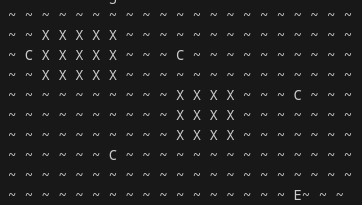
\includegraphics[width=\textwidth]{dev-python/terrain1.png}
        \caption{Terrain sans réseau}
        \label{fig:image1}
    \end{minipage} \hfill
    \begin{minipage}{0.48\textwidth}
        \centering
        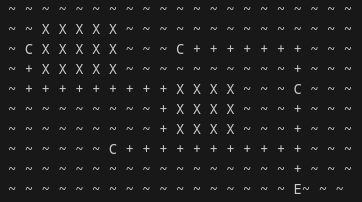
\includegraphics[width=\textwidth]{dev-python/terrain2.png}
        \caption{Réseau après BFS}
        \label{fig:image2}
    \end{minipage}
\end{figure}

\subsection{Écriture des tests}

Après avoir terminé l'implémentation des fonctions, nous avons développé des tests unitaires pour en valider le comportement. Ces tests ont permis de s’assurer que chaque fonction répond correctement aux différents cas d’utilisation, y compris les situations limites.

L’écriture de ces tests a également joué un rôle clé dans la détection précoce d’éventuelles erreurs, tout en garantissant une base solide pour les étapes suivantes du projet. Cette démarche a renforcé la fiabilité globale du code et assuré une meilleure maintenance.

